\section{Stima della corrente di attivazione}

\begin{wrapfigure}[14]{r}[0pt]{100mm}
	\centering
    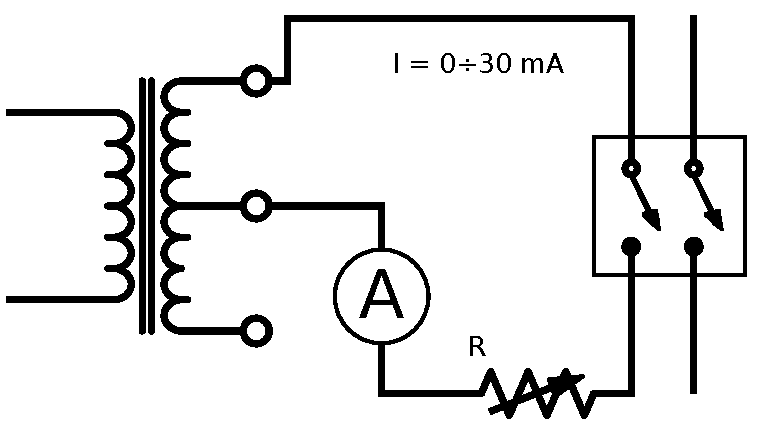
\includegraphics[width=0.40\textwidth]{amper.pdf}
    \caption{Schema del circuito utilizzato per la misura differenziale di corrente.}
    \label{fig:amper}
\end{wrapfigure}

L'interruttore differenziale sfrutta l'induzione magnetica per rilevare perdite di corrente e intervenire aprendo il circuito. Esso ha al suo interno due bobine avvolte in modo che, quando il circuito funziona correttamente, ovvero la corrente in uscita eguaglia la corrente in entrata, i campi magnetici generati dalle bobine si annullano a vicenda. Quando invece si ha una perdita di corrente (ad esempio a terra), i campi magnetici generati sono diversi e si ha dunque un effetto di induzione elettromagnetica su una terza bobina che, attivando un meccanismo, apre il circuito.

Come mostrato in Fig. \ref{fig:amper}, abbiamo montato il circuito facendo passare un solo cavo nell'interruttore differenziale. Così facendo, abbiamo simulato il caso in cui la perdita di corrente è del 100\% a terra. Misurando poi, attraverso il multimetro, per quale valore di corrente l'interruttore scattava e ripetendo le misure varie volte, abbiamo stimato un valore di corrente di attivazione. 

Avendo alimentato il circuito con una tensione alternata a $7.5V_{rms}$, abbiamo utilizzato una decade di resistenze per poter ottenere diversi valori di corrente nel circuito. Sono stati eseguiti 15 campionamenti, con valor medio di $(26.5\pm0.3)\si{\milli\ampere}$. Abbiamo osservato che il valore di corrente di attivazione si aveva per un valore di resistenza di circa $300\si{\ohm}$. 


\section{Stima del tempo di intervento}

\begin{wrapfigure}[14]{r}[0pt]{100mm}
	\centering
    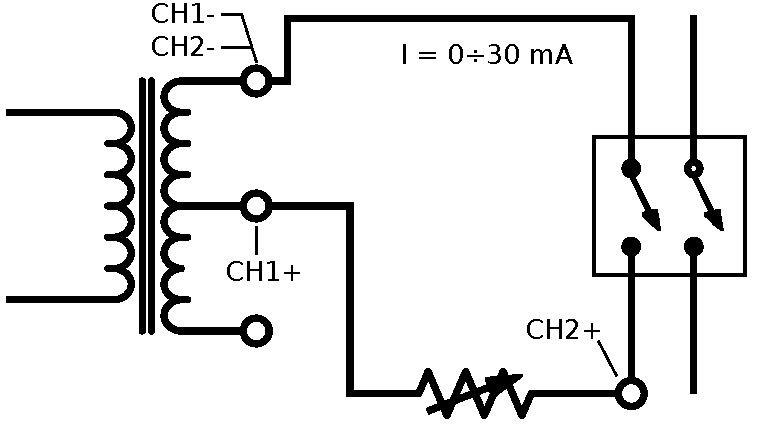
\includegraphics[width=0.40\textwidth]{time.pdf}
    \caption{Schema del circuito utilizzato per la stima del tempo di intervento.}
    \label{fig:time}
\end{wrapfigure}

Per stimare il tempo di intervento dell'interruttore abbiamo utilizzato l'oscilloscopio in modalità acquisizione singola. In questa modalità lo strumento inizia a prendere dati solo nel momento in cui rileva un segnale, facendone un'istantanea sullo schermo. Risulta così possibile osservare un fenomeno isolato e non periodico bloccandone l'immagine e analizzandola successivamente.

Come mostrato in Fig. \ref{fig:time}, sono stati collegati i canali dell'oscilloscopio in modo da avere sullo schermo sempre il segnale ai capi del generatore di tensione e quello ai capi dell'interruttore differenziale. Così facendo, fino a quando l'interruttore differenziale rimane chiuso, la ddp ai suoi capi sarà nulla mentre dopo l'apertura osserveremo un andamento identico a quello in input.

Per stimare il tempo di intervento abbiamo spento il generatore di tensione, impostata una resistenza bassa (inferiore a quella di soglia stimata nella sezione precedente) e chiuso l'interruttore. Dopo aver impostato l'oscilloscopio in acquisizione singola, abbiamo acceso il generatore di tensione. Sullo schermo abbiamo ottenuto una figura come quella riportata in Fig. \ref{fig:graph}.

\begin{figure}[h]
	\centering
    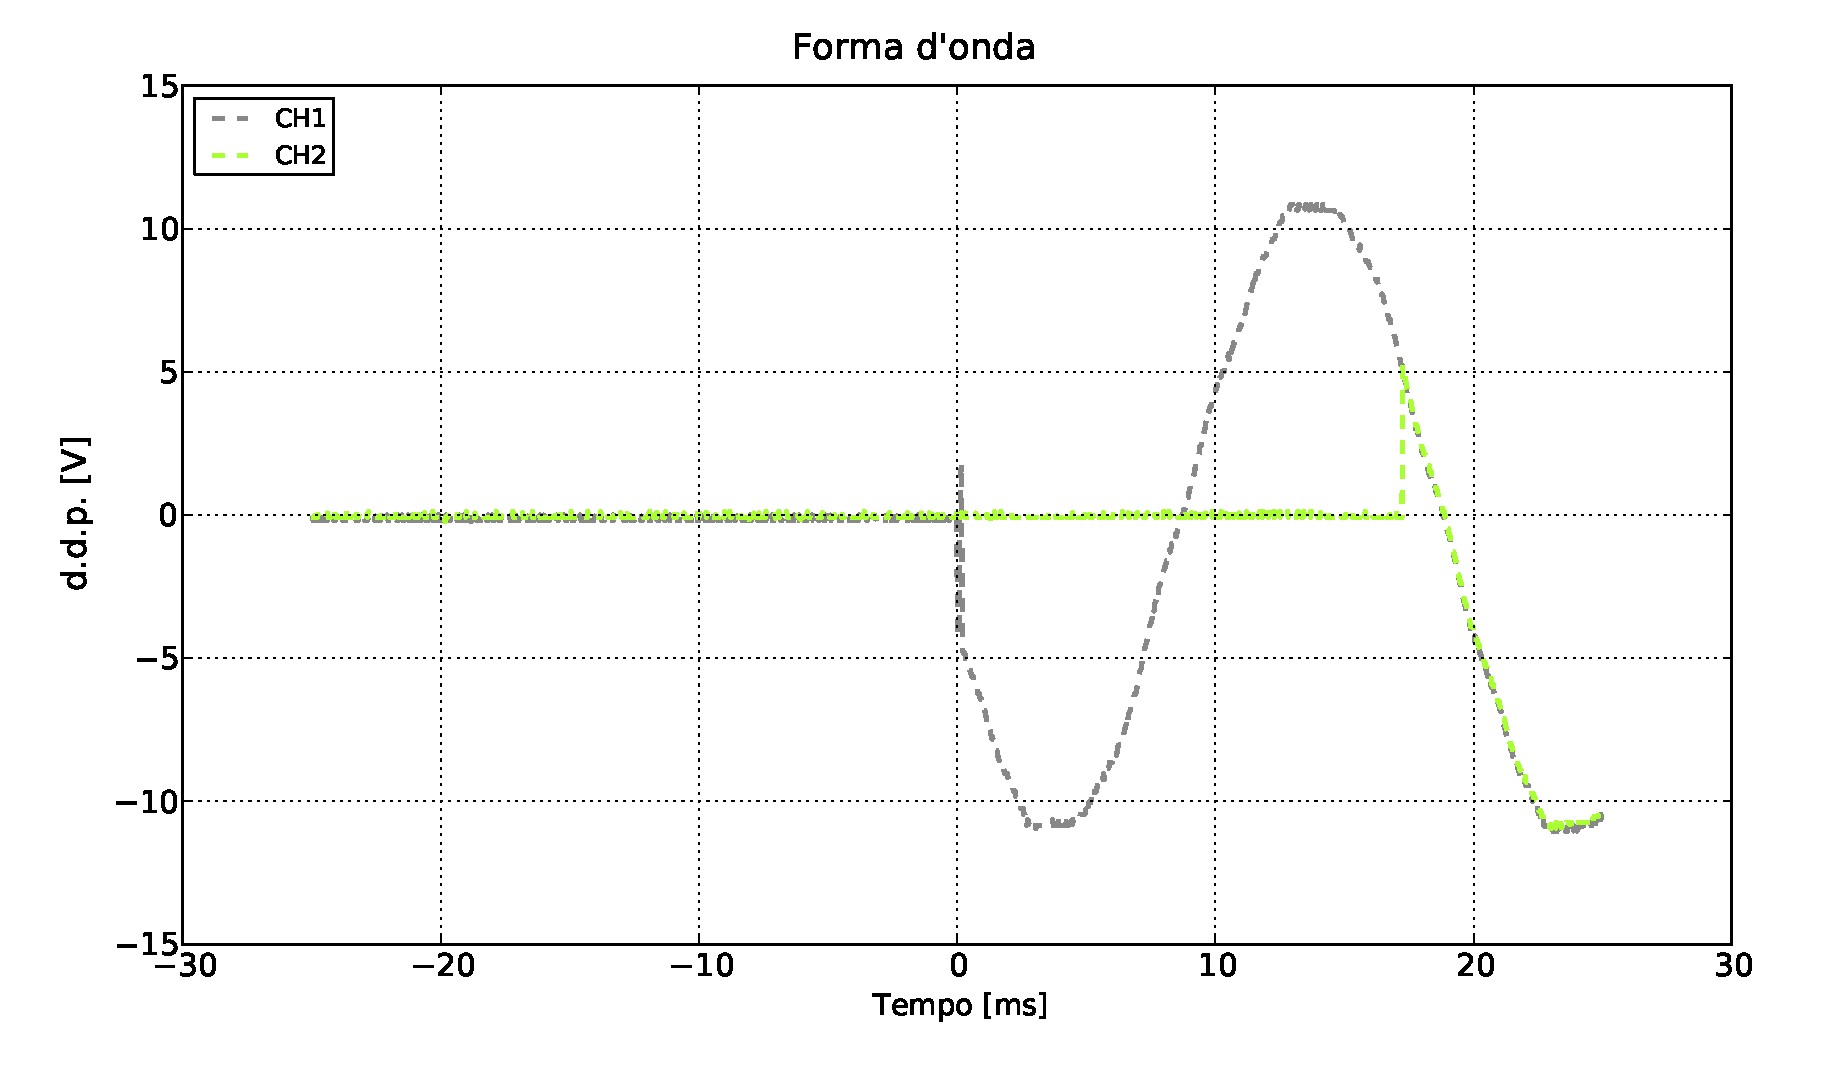
\includegraphics[height=3in]{graph.pdf}
    \caption{Grafico rappresentante la visualizzazione a schermo della d.d.p. tra i \emph{jack} dei due canali rilevati dall'oscilloscopio.}
    \label{fig:graph}
\end{figure}


Utilizzando i puntatori sullo schermo, abbiamo stimato il valore di $\Delta t$ che intercorreva tra il momento di accensione del generatore (quando compare il segnale sullo schermo riferito al CH1) e il momento in cui lo stesso segnale appariva su CH2. Abbiamo notato che tale intervallo di tempo era fortemente variabile (anche $10\si{\milli\second}$ per lo stesso valore di resistenza). Inoltre, provando con diversi valori di resistenza $R$ si è notato che mediamente il tempo di intervento aumentava. Sono stati eseguiti 5 campionamenti per ciascuna resistenza. Riportiamo in tabella i valori medi di tempo di intervento.

\begin{table}[h]
\centering
\caption{estiqatsi}
{\renewcommand{\arraystretch}{1.6}%
\begin{tabular}{c|c|c|c|c}
 & $R=50 \si{\ohm}$ & $R=100 \si{\ohm}$ & $R=200 \si{\ohm}$ & $R=250 \si{\ohm}$ \\      \hline
$t_{att}$ [$\si{\milli\second}$] & $(3.4 \pm 0.1)$ & $(3.7 \pm 0.2)$ & $(3.5 \pm 0.2)$ & ($3.5 \pm 0.1$) \\
\end{tabular}}
\end{table}


Abbiamo casualmente notato che, sebbene i tempi di attivazione a parità di resistenza fossero diversi, il tempo tra l'ultimo passaggio del segnale sull'asse delle $x$ e l'apertura dell'interruttore rimaneva costante. Abbiamo dunque ipotizzato l'esistenza di un tempo di attivazione ``meccanico'' (ovvero dal momento in cui l'interruttore sente la differenza di corrente critica e inizia il processo meccanico di apertura del circuito fino al completamento dello stesso), fosse una costante (che chiameremo $\tau$).  Riportiamo i tempi tra ultimo passaggio del segnale sull'asse $x$ e apertura del circuito nella seguente tabella. 

\begin{table}[h]
\centering
\caption{estiqatsi}
{\renewcommand{\arraystretch}{1.6}%
\begin{tabular}{c|c|c|c|c}
 & $R=50 \si{\ohm}$ & $R=100 \si{\ohm}$ & $R=200 \si{\ohm}$ & $R=250 \si{\ohm}$ \\      \hline
$\Delta t$ [$\si{\milli\second}$] & $(3.4 \pm 0.1)$ & $(3.7 \pm 0.2)$ & $(3.5 \pm 0.2)$ & ($3.5 \pm 0.1$) \\
\end{tabular}}
\end{table}

Come vediamo, i valori variano al variare della resistenza. Ciò è coerente con il fatto che a parità di tensione, con resistenze più alte scorre meno corrente. Inoltre, l'interruttore differenziale sfrutta le variazioni di corrente, pertanto esso sarà sensibile alla derivata della corrente.

Assumendo una forma della corrente\footnote{Per comodità immaginiamo di eseguire una traslazione in modo che la fase $\varphi$ sia uguale a zero.}:
\begin{equation}
I(t)=\frac{V_0}{R}sin(\omega t)
\label{corrente}
\end{equation}

Risulta banale calcolare la sua derivata temporale:

\begin{equation}
\frac{dI(t)}{dt}=\frac{V_0 \omega}{R}cos(\omega t)
\end{equation}

La corrente indotta nell'interruttore differenziale sarà dunque proporzionale alla derivata temporale della corrente moltiplicata per una costante, che tiene conto delle geometrie dello strumento stesso. L'interruttore avrà una corrente di attivazione $I_a=cost$. Possiamo dunque scrivere la seguente relazione:

\begin{equation}
\frac{V_0 \omega}{R}cos(\omega t)=I_a \Rightarrow t=\frac{acos(\frac{I_a R}{\omega V_0})}{\omega }
\label{oi}
\end{equation} 

Abbiamo dunque stimato che il tempo di reazione meccanico dello strumento non può essere inferiore alla somma di $\Delta t$ e del $t$ calcolato tramite eq. (\ref{oi}), in quanto $\Delta t$ era una costante sempre a parità di resistenza e tutti i campionamenti effettuati avevano almeno un massimo prima del passaggio della della tensione sullo zero. Abbiamo dunque imposto la condizione 
